\documentclass[a4paper,
fontsize=11pt,
%headings=small,
oneside,
numbers=noperiodatend,
parskip=half-,
bibliography=totoc,
final
]{scrartcl}

\usepackage[babel]{csquotes}
\usepackage{synttree}
\usepackage{graphicx}
\setkeys{Gin}{width=.4\textwidth} %default pics size

\graphicspath{{./plots/}}
\usepackage[ngerman]{babel}
\usepackage[T1]{fontenc}
%\usepackage{amsmath}
\usepackage[utf8x]{inputenc}
\usepackage [hyphens]{url}
\usepackage{booktabs} 
\usepackage[left=2.4cm,right=2.4cm,top=2.3cm,bottom=2cm,includeheadfoot]{geometry}
\usepackage{eurosym}
\usepackage{multirow}
\usepackage[ngerman]{varioref}
\setcapindent{1em}
\renewcommand{\labelitemi}{--}
\usepackage{paralist}
\usepackage{pdfpages}
\usepackage{lscape}
\usepackage{float}
\usepackage{acronym}
\usepackage{eurosym}
\usepackage{longtable,lscape}
\usepackage{mathpazo}
\usepackage[normalem]{ulem} %emphasize weiterhin kursiv
\usepackage[flushmargin,ragged]{footmisc} % left align footnote
\usepackage{ccicons} 
\setcapindent{0pt} % no indentation in captions

%%%% fancy LIBREAS URL color 
\usepackage{xcolor}
\definecolor{libreas}{RGB}{112,0,0}

\usepackage{listings}

\urlstyle{same}  % don't use monospace font for urls

\usepackage[fleqn]{amsmath}

%adjust fontsize for part

\usepackage{sectsty}
\partfont{\large}

%Das BibTeX-Zeichen mit \BibTeX setzen:
\def\symbol#1{\char #1\relax}
\def\bsl{{\tt\symbol{'134}}}
\def\BibTeX{{\rm B\kern-.05em{\sc i\kern-.025em b}\kern-.08em
    T\kern-.1667em\lower.7ex\hbox{E}\kern-.125emX}}

\usepackage{fancyhdr}
\fancyhf{}
\pagestyle{fancyplain}
\fancyhead[R]{\thepage}

% make sure bookmarks are created eventough sections are not numbered!
% uncommend if sections are numbered (bookmarks created by default)
\makeatletter
\renewcommand\@seccntformat[1]{}
\makeatother

% typo setup
\clubpenalty = 10000
\widowpenalty = 10000
\displaywidowpenalty = 10000

\usepackage{hyperxmp}
\usepackage[colorlinks, linkcolor=black,citecolor=black, urlcolor=libreas,
breaklinks= true,bookmarks=true,bookmarksopen=true]{hyperref}
\usepackage{breakurl}

%meta
%meta

\fancyhead[L]{D. Göhring\\ %author
LIBREAS. Library Ideas, 39 (2021). % journal, issue, volume.
\href{https://doi.org/10.18452/23447}{\color{black}https://doi.org/10.18452/23447}
{}} % doi 
\fancyhead[R]{\thepage} %page number
\fancyfoot[L] {\ccLogo \ccAttribution\ \href{https://creativecommons.org/licenses/by/4.0/}{\color{black}Creative Commons BY 4.0}}  %licence
\fancyfoot[R] {ISSN: 1860-7950}

\title{\LARGE{Begegnung der anderen Art: Roboter in deutschen Bibliotheken}}% title
\author{Dominic Göhring} % author

\setcounter{page}{1}

\hypersetup{%
      pdftitle={Begegnung der anderen Art: Roboter in deutschen Bibliotheken},
      pdfauthor={Dominic Göhring},
      pdfcopyright={CC BY 4.0 International},
      pdfsubject={LIBREAS. Library Ideas, 39 (2021).},
      pdfkeywords={Roboter, Künstliche Intelligenz, Bibliotheken, Deutschland},
      pdflicenseurl={https://creativecommons.org/licenses/by/4.0/},
      pdfcontacturl={http://libreas.eu},
      baseurl={https://doi.org/10.18452/23447},
      pdflang={de},
      pdfmetalang={de}
     }



\date{}
\begin{document}

\maketitle
\thispagestyle{fancyplain} 

%abstracts
\begin{abstract}
\noindent
\textbf{Kurzfassung:} Der Beitrag begibt sich auf Spurensuche und versucht einen Überblick zu
geben, in welcher Funktion Roboter in deutschen Bibliotheken eingesetzt
werden, wie Roboter von Nutzenden und Belegschaft angenommen werden und
was die Grenzen des Einsatzes der Bibliotheksrobotik sind. Dazu wurden
vier Einrichtungen in einem schriftlichen beziehungsweise telefonischen
Interview zu den sich im Einsatz befindlichen Robotern befragt und die
Ergebnisse in dieser Umfrage dargestellt.

\noindent\textbf{Schlüsselwörter:} Roboter, Künstliche Intelligenz, Bibliotheken,
Deutschland
\end{abstract}

%body

\begin{figure}[]
\centering
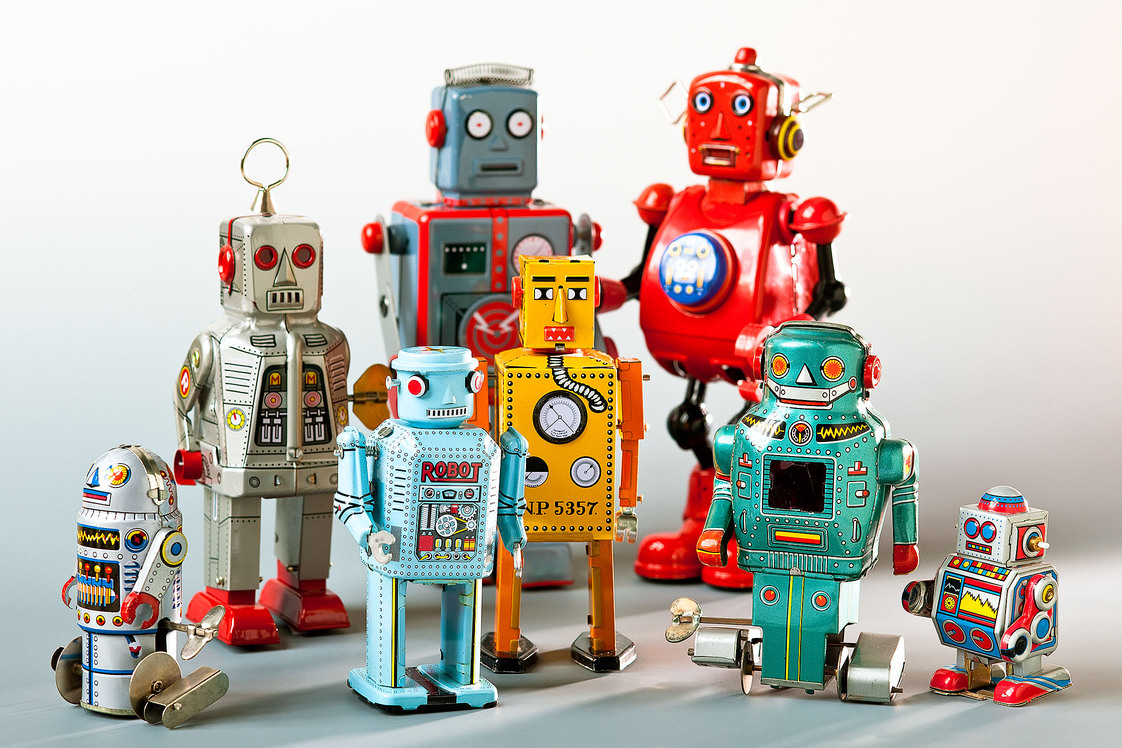
\includegraphics[width=.7\textwidth]{img/Robotervitrine.jpg}
\caption{Roboter aus der Robotervitrine im Eingangsbereich des Deutsches
Technikmuseum in Berlin. {[}Mit freundlicher Genehmigung der Stiftung Deutsches Technikmuseum Berlin (Bildrechte: SDTB / C. Kirchner).{]}}
\end{figure}

Während des Semesterstarts ist an Universitäten bekanntlich viel los.
Überall herrscht hektische Betriebsamkeit. Studierende suchen ihren
Vorlesungsraum oder einen Essensplatz in der -- wie immer viel zu vollen
-- Mensa. Auch in den Universitätsbibliotheken herrscht Hochbetrieb.
Studierende besuchen Führungen und Einführungskurse, um die Räume und
Services der Bibliothek kennenzulernen. Seit vielen Jahren findet man im
September immer wieder ein ähnliches Bild vor. Doch an immer mehr
Einrichtungen werden die Studierenden nicht mehr von der netten
Bibliothekarin oder dem freundlichen Bibliothekar durch die Bibliothek
geführt, sondern von kindsgroßen humanoiden Robotern, die zum Beispiel
auf den Namen Wilma, Ada oder Nao hören.

Als ich mich auf die Suche nach Robotern in deutschen Bibliotheken
mache, bin ich erstaunt, wie groß die Bandbreite der im Einsatz
befindlichen Bibliotheksroboter ist. Und das betrifft nicht nur die
äußere Erscheinung (wie Größe, Form und Ausstattung), sondern auch die
vielfältigen Einsatzgebiete und das Aufgabenspektrum, welche die
Maschinen in der Bibliothek übernehmen vom Transport von Büchern über
das Durchführen von Führungen bis hin zum mobilen Informationssystem.

\hypertarget{fragestellungen}{%
\section{Fragestellungen}\label{fragestellungen}}

Im ersten Teil des Beitrags werde ich der Frage nachgehen, welche
Funktion ein Roboter in einer Bibliothek erfüllt. Interessant ist dabei
vor allem die Fragestellung, von welchen Aufgaben der Roboter die
Bibliotheksmitarbeitenden \enquote{befreien} und entlasten soll und in
welcher Art und Weise er die Belegschaft sogar ersetzen kann oder soll.
Sind dies lediglich monotone beziehungsweise iterative Arbeiten wie
beispielsweise die Bibliotheksinventur und körperlich anstrengende
Arbeiten wie der Transport von Büchern? Oder soll der Roboter den
Bibliotheksmitarbeitenden auch in Hinblick auf Dienste und Services mehr
und mehr substituieren, ganz gemäß der Erfüllung des Bedürfnisses des
Nutzenden nach einer Verfügbarkeit von Angeboten nach der Maxime 24/7?
Der zweite Teil des Beitrags beschäftigte sich mit den Grenzen des
Einsatzes von Bibliotheksrobotern. Welche Schwierigkeiten und Probleme
bringt ihr Einsatz im realen, materiellen Raum mit sich? Damit verbunden
stellt sich auch die Frage, ob in Bibliotheken der Einsatz einer anderen
Art von Maschine beziehungsweise Technologie, nämlich die des Computers
-- welche im virtuellen und nichtmateriellen Raum agiert -- nicht einen
größeren Mehrwert verspricht als ein Roboter. Stichworte sind in diesem
Zusammenhang Begriffe wie Künstliche Intelligenz, Maschinelles Lernen
und computerbasierte Wissens- und Informationsvernetzung.

Der dritte Teil des Beitrags setzt sich mit der Frage auseinander, wie
der Mensch mit dem \enquote{Humanoiden} umgeht. Tritt man diesem
aufgeschlossen oder zurückhaltend gegenüber, gibt es Berührungsängste
von Seiten der Nutzenden und wie gestaltet sich der Erstkontakt mit dem
Roboter? Mich interessiert auch die Sicht der Belegschaft auf den/die
Kolleg*innen der anderen Art. Wird der Roboter als Konkurrenz angesehen
oder als Kolleg*in, der/die ungeliebte Arbeiten oder Routineaufgaben
abnimmt und welcher es ermöglicht, sich auf interessantere und
wichtigere Aufgaben oder Projekte zu konzentrieren?

\hypertarget{methode}{%
\section{Methode}\label{methode}}

Es wurden vier Einrichtungen (zwei Wissenschaftliche Bibliotheken und
zwei Öffentliche Bibliotheken) kontaktiert, welche Roboter in ihrer
Bibliothek im Einsatz haben. In einem schriftlichen beziehungsweise
telefonischen Interview habe ich um die Beantwortung der oben genannten
Fragen gebeten. Es folgt ein Überblick über die Antworten der
Einrichtungen.

\hypertarget{funktion-von-robotern-in-uxf6ffentlichen-bibliotheken}{%
\section{Funktion von Robotern in Öffentlichen
Bibliotheken}\label{funktion-von-robotern-in-uxf6ffentlichen-bibliotheken}}

\begin{figure}
\centering
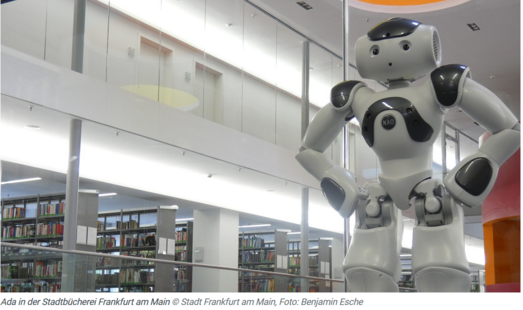
\includegraphics[width=.7\textwidth]{img/ADA.PNG}
\caption{ADA in der Stadtbücherei Frankfurt am Main {[}© Stadt Frankfurt am Main, Foto: Benjamin Esche, mit freundlicher Genehmigung der Stadtbücherei Frankfurt am Main{]}}
\end{figure}

Die Stadtbücherei Frankfurt am Main und die Stadtbibliothek Köln setzen
beide einen humanoiden Roboter namens ADA beziehungsweise NAO als Lern-
und Demonstrationsobjekt ein. Beide Einrichtungen definieren ihre
Aufgabe darin, den umfassenden Zugang zu Medien und Technologien aller
Art -- und dazu gehören auch Roboter -- zu ermöglichen. Die Roboter
haben die Funktion, die Begegnung mit einer neuen Technik auf eine
spielerische Art und Weise zu ermöglichen. So sollen die Nutzenden von
Kinderschuhen an bis ins Erwachsenenalter auf unterhaltsame und
experimentelle Art und Weise an das Thema Programmierung und Robotics
herangeführt werden. Die Nutzenden können die Roboter über ein Tablet
steuern und mit ihnen sprechen oder Informationen zu den Services und
Benutzungsmodalitäten der Bibliothek abrufen. Frauke Buhlmann von der
Stadtbibliothek Köln erzählt mir: \enquote{Mit den Robotern finden auch
Vorführungen und Animationen statt, um es den Nutzenden zu ermöglichen,
mit den Robotern zu interagieren; sie können dann Fragen stellen
beziehungsweise High Five mit NAO machen. Darüber hinaus finden
regelmäßig Programmierworkshops statt, welche der Zugänglichmachung der
neuen Technologie des Roboters und ein unmittelbares Erlebnis und
Auseinandersetzen mit dieser ermöglichen sollen.}\footnote{Schriftliches
  Interview mit Frauke Buhlmann (Stadtbibliothek Köln), geführt am 21.
  Dezember 2020.} Durch den direkten Kontakt mit den Robotern sollen die
Nutzenden mit dem Thema Robotics in Berührung gebracht und so ein
gesellschaftlicher Diskurs angestoßen werden.

In einem YouTube Video\footnote{Stadtbücherei Frankfurt am Main: Hello
  World - ADA, Dash \& Co.~stellen sich vor
  \url{https://www.youtube.com/watch?v=NMUsmLztOCo} (aufgerufen am
  7.4.2021).} der Stadtbücherei Frankfurt werden noch weitere Lern- und
Demonstrationsroboter (Dash, Ozobot Evos, Blue Bot und Thymio)
beziehungsweise Anwendungsroboter wie DOBOT vorgestellt, welche eine
ähnliche Aufgabe wie ADA oder NAO haben. Auch sie sollen die Nutzenden
mit \enquote{Spaß und Kreativität an das Programmieren, das sogenannte
Coding, heranführen.}\footnote{Stadtbücherei Frankfurt am Main: Hello
  World - ADA, Dash \& Co.~stellen sich vor
  \url{https://www.youtube.com/watch?v=NMUsmLztOCo} (aufgerufen am
  7.4.2021).} Die Öffentlichen Bibliotheken
erfüllen in diesem Zusammenhang eine gesellschaftliche Aufgabe und
Verantwortung. Sie ermöglichen es, als Orte der Begegnung und des
Austausches einen Raum bereitzustellen, um sich mit neuen Technologien
(Automatisierung, Digitalisierung und Robotik), welche das gesamte
gesellschaftliche Leben beeinflussen, auf informeller Ebene und durch
einen niedrigschwelligen Zugang auseinanderzusetzen. Frauke Buhlmann
erzählt mir weiter: \enquote{An die Interaktion mit den Robotern wird
somit spielerisch, informativ und experimentell
herangeführt.}\footnote{Schriftliches Interview mit Frauke Buhlmann
  (Stadtbibliothek Köln), geführt am 21. Dezember 2020.}

Die Öffentlichen Bibliotheken ermöglichen die Begegnung mit den Robotern
aber nicht nur innerhalb der eigenen Einrichtung, sondern sie beteiligen
sich beispielsweise auch an Initiativen wie: \enquote{‚Digital für
alle': Digitale Teilhabe jetzt umfassend ermöglichen!}\footnote{Appell
  der Initiative \enquote{Digital für alle}: Digitale Teilhabe jetzt
  umfassend ermöglichen! \url{https://digitaltag.eu/appell} (aufgerufen
  am 7.4.2021).} Ziel des Zusammenschlusses von 27 Organisationen aus
Zivilgesellschaft, Kultur, Wissenschaft, Wirtschaft und öffentlicher
Hand ist es, durch einen bundesweiten \enquote{Digitaltag} Räume des
Erlebens und des Kontaktes mit digitalen Technologien zu schaffen. So
soll der zunehmenden digitalen Spaltung breiter Bevölkerungsschichten
entgegengewirkt werden, indem digitale Kompetenzen vermittelt und die
Gesellschaft auf die neuen (digitalen) Herausforderungen beruflicher
oder privater Natur vorbereitet werden.

Auch die Stadtbücherei Frankfurt hat in diesem Zusammenhang ihre Roboter
vorgestellt und versucht so, Themen wie Digitalisierung und Roboter mehr
in die \enquote{Mitte der Gesellschaft} zu rücken, und zwar in einer
plastischen und erlebbaren Form. Elfriede Ludwig, die Leiterin des
Bereichs \enquote{Digitale Dienste} in der Stadtbücherei Frankfurt am Main,
meint in diesem Zusammenhang: 

\begin{quote}
\enquote{Wie könnte man Themen wie
Robotik, Coding und Programmieren besser erfahrbar machen als am Roboter
selbst? Diese Gedanken haben uns am Ende dazu bewogen, Roboter
anzuschaffen {[}\ldots{]}.}\footnote{Ludwig, Elfriede: Roboter gehören
  in eine Öffentliche Bibliothek. In: Forum Bibliothek und Information
  11/2019, Seite S. 621 und 622.} 
 \end{quote}
  
Als informelle Bildungseinrichtungen
sollen Bibliotheken so helfen, ergänzend zu den schulischen Angeboten,
eine Plattform zu bieten, um Zugänge zu schaffen, sich mit neuen
Technologien zu konfrontieren und kritisch auseinanderzusetzen. All dies
in der Hoffnung, so die Lücke der digitalen Spaltung der Gesellschaft zu
verkleinern. In dieser Funktion wollen Bibliotheken eine wichtigen
Beitrag bei der Partizipation und Teilhabe breiter Bevölkerungsschichten
am digitalen Wandel des gesamten gesellschaftlichen und öffentlichen
Lebens leisten. Der Roboter soll zum einen praktischen Wert haben, zum anderen
aber auch erfreuen, ganz im Sinne des aufklärerischen Grundsatzes
\enquote{Prodesse et delectare}. Bibliotheken sind in dieser Funktion
Erkundungs- und Experimentierort, an dem man Wissen vermittelt, das
sinnlich erfahrbar und erlebbar ist. Digitales Mindset ist das
Schlagwort der Stunde. Und Roboter sind innerhalb dieses Prozesses von
der Transformation traditioneller Wissensvermittlung zu anregenden,
inspirierenden und lernfördernden Formen in Öffentlichen Bibliotheken
ein Mittel der Wahl.

\hypertarget{funktion-von-robotern-in-wissenschaftlichen-bibliotheken}{%
\section{Funktion von Robotern in Wissenschaftlichen
Bibliotheken}\label{funktion-von-robotern-in-wissenschaftlichen-bibliotheken}}

\begin{figure}
\centering
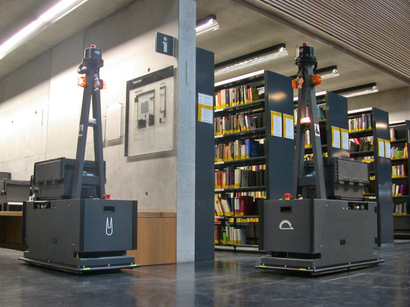
\includegraphics[width=.7\textwidth]{img/HaseIgel.png}
\caption{Transportroboter Hase und Igel in der Zweigbibliothek
Naturwissenschaften. {[}Foto mit freundlicher Genehmigung der
Universitätsbibliothek der Humboldt-Universität zu Berlin, \href{https://creativecommons.org/licenses/by/4.0/}{CC BY 4.0} UB der
HU Berlin, Anja Herwig{]}}
\end{figure}

Ganz im Gegensatz zu den Vertretern der Öffentlichen Bibliotheken haben
sich die befragten Wissenschaftlichen Bibliotheken eher aus praktischen
Gründen für die Anschaffung und den Einsatz eines Bibliotheksroboters
entschieden. In der Universitätsbibliothek der Humboldt-Universität zu
Berlin, Zweigbibliothek Naturwissenschaften im
Erwin-Schrödinger-Zentrum, begegnen einem seit 2003 zwei baugleiche
Fahrzeuge eines fahrerlosen Transportsystems, die von den Mitarbeitenden
auf den Namen \enquote{Hase \& Igel} getauft wurden. Die beiden
Blechkollegen haben die Aufgabe, die Buchtransporte innerhalb der
Bibliothek zu übernehmen. Eigentlich sollte eine unterirdische Anlage
den Transport der Medien ausgehend von der Ausleih- und Rückgabetheke
übernehmen. Geologische Bedingungen machten diese Lösung des
Medientransports allerdings unmöglich. Die Bibliothek musste somit über
eine alternative Möglichkeit nachdenken, die Bücher innerhalb der
Einrichtung an die entsprechende Stelle zu befördern. Eine Hamburger
Firma, spezialisiert auf Transport-Robotik, brachte den entscheidenden
Durchbruch, indem sie ihre Roboter an die Anforderungen der Bibliothek
anpasste. Trotz des Publikumsverkehrs in der Bibliothek wurde es damit
möglich, dass die Roboter bei entsprechendem Auftrag Buchkisten
aufnehmen und sich den Weg durch eine staunende Öffentlichkeit bahnen,
bis sie an ihrem Zielort angekommen sind. \enquote{In Anlehnung an das
Grimm'sche Märchen vom ewigen Wettlauf zwischen Hase und
Igel}\footnote{Schulz, Eckart: Der ewige Wettlauf zwischen Hase und Igel.
  In: Forum Bibliothek und Information 02-03/2018, Seite 114\emph{.}}
werden so seit 2003 die Medien in Adlershof an die entsprechende Stelle
transportiert, erzählt mir Anja Herwig, die stellvertretende Leiterin
der Zweigbibliothek Naturwissenschaften. Allerdings ziehen die Roboter
immer weniger ihre Runden durch die einprogrammierten Laufwege der
Bibliothek. \enquote{Die beiden Blechkollegen sind schon etwas in die
Jahre gekommen und laufen nicht mehr ganz störungsfrei},\footnote{Schriftliches
  Interview mit Anja Herwig (stellvertretende Leiterin der
  Zweigbibliothek Naturwissenschaften der Humboldt-Universität zu
  Berlin), geführt am 13. Januar 2021.} resümiert sie weiter. Und da
die beiden Exoten einzigartig in der Bibliothekslandschaft sind,
scheitere es zunehmend an der Beschaffung von Ersatzteilen
beziehungsweise an Techniker*innen, welche die Montage und Reparaturen
vornehmen können. Und so ruhen sich \enquote{Hase \& Igel} immer
häufiger im sogenannten Schlafzimmer aus und ziehen nur noch zu
besonderen Anlässen (zum Beispiel beim Besuch hoher Politiker*innen)
ihre Bahnen durch die Bibliothek.

Nur wenige Kilometer von Adlershof entfernt begegnet man in der
Hochschulbibliothek der Technischen Hochschule Wildau einem humanoiden
Roboter des Typs Pepper. Wilma ist aber nicht alleine nach Wildau
gekommen, sondern hat Verstärkung mitgebracht. Ihr \enquote{Alter Ego}
steht als Testinstanz im Fachbereich Telematik der TH Wildau. An ihm
können die Studierenden die Anwendungen ausprobieren, welche Wilma im
Produktivbetrieb in der Hochschulbibliothek seit 2017 umsetzen soll.
Dirk Wissen, BuB-Herausgeber, führte 2018 ein Interview mit Wilma. In
dem Video\footnote{Auf einen Espresso mit Wilma -- Interview mit dem
  humanoiden Roboter Pepper
  \url{https://www.youtube.com/watch?v=-gGQBuOBg7U} (aufgerufen am
  7.4.2021).} definiert die Roboterdame ihre Aufgabe und Funktion
innerhalb der Bibliothek wie folgt:

\begin{quote}
\enquote{Ich verstehe mich eher als Assistenzsystem und helfe den
Mitarbeiter*innen der Bibliothek, wo ich kann und bringe ihnen
Entlastung. Ich bin ein Lern- und Forschungsroboter; das heißt, die
Studenten des Studiengangs Telematik, die mich vorwiegend programmieren,
probieren viel an mir aus -- was als Ergebnis den Kunden der Bibliothek
zugute kommen soll {[}\ldots{]}. Ich unterstütze zum Beispiel, indem ich
kleine Bibliotheksführungen gebe oder Zuhörern zum Entspannen Witze
erzähle, mit -- vor allem jungem -- Nachwuchs Schere-Stein-Papier spiele
oder für ein Selfie zur Verfügung stehe. Ab dem kommenden Wintersemester
soll ich helfen, das Fehlen von Fachpersonal in den Abend- und
Morgenstunden zu kompensieren, damit Studierende rund um die Uhr hier
arbeiten können.}\footnote{Auf einen Espresso mit Wilma -- Interview
  mit dem humanoiden Roboter Pepper
  \url{https://www.youtube.com/watch?v=-gGQBuOBg7U} (aufgerufen am
  7.4.2021).}
\end{quote}

\begin{figure}
\centering
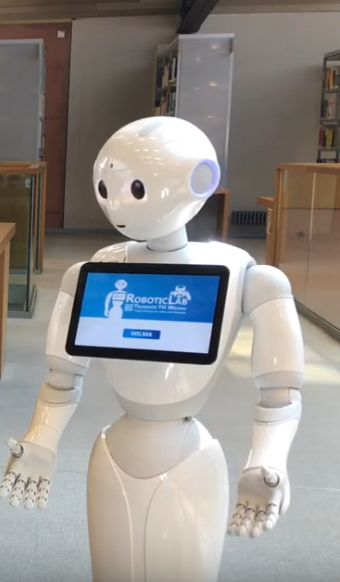
\includegraphics{img/Wilma.PNG}
\caption{Screenshot aus dem Video: Auf einen Espresso mit Wilma. {[}Mit freundlicher Genehmigung der Hochschulbibliothek der TH Wildau (Dr. Frank Seeliger).{]}}
\end{figure}

Im Konzept bezüglich der Einsatzgebiete von Wilma sei immer angelegt
gewesen, so sagt mir der Bibliotheksdirektor der Hochschulbibliothek der
Technischen Hochschule Wildau, Dr.~Frank Seeliger, dass der Roboter für
die Öffnung der Bibliothek (24/7) vorgesehen ist. Die Nutzenden sollten
auch außerhalb der Öffnungszeiten mit einer Chipkarte in die Bibliothek
kommen können. Allerdings wollte man ihnen den Bibliotheksraum nicht
gänzlich alleine überlassen, sondern ihnen \enquote{ein System an die
Seite stellen, was ihnen bei Fragen oder Problemen hilft. Und in dieser
Funktion kam Wilma ins Spiel. Sie sollte von 20 Uhr bis morgens um 9 Uhr
diese Lücke an fehlendem Fachpersonal füllen.}\footnote{Telefonisches
  Interview mit Dr.~Frank Seeliger (Leiter der Hochschulbibliothek der
  TH Wildau), geführt am 21. Dezember 2020.} Als Assistenzsystem sollte
Wilma bei Fragen zu den Services und der Funktionsweise der Bibliothek
Hilfestellung geben oder mit den Nutzenden in Interaktion treten können.
Hierzu hätte insbesondere die Lokalisierung und Ermahnung von zu lauten
Bibliotheksbesuchern oder die Auflockerung des Besuchs durch das
Erzählen eines Witzes gezählt. Des Weiteren sollte Wilma den Nutzenden
bei der Navigation und Orientierung im Raum unterstützen; beispielsweise
helfen, ein bestimmtes Buch zu lokalisieren und den Nutzenden dorthin zu
navigieren. Außerdem sollten Dienstleistungen wie die Ausgabe und
Rückgabe von Büchern über den Roboter möglich sein. So weit so schön in
der Theorie.

\hypertarget{schwierigkeiten-und-probleme-von-bibliotheksrobotern}{%
\section{Schwierigkeiten und Probleme von
Bibliotheksrobotern}\label{schwierigkeiten-und-probleme-von-bibliotheksrobotern}}

In der Praxis habe es allerdings erhebliche Probleme gegeben, welche man
nicht komplett lösen könne, erzählt mir Seeliger. Die Schwierigkeiten
basierten hauptsächlich auf den Gegebenheiten der Bibliothek, die es dem
Roboter erschwerten, sich ungehindert durch die Bibliothekräume zu
bewegen. So war es für Wilma schwierig, den Fahrstuhl zu benutzen, um
von einer Etage auf die andere zu gelangen und auch Parameter wie
Lichtverhältnisse und Störgeräusche beeinträchtigten die Indoor
Navigation. Des Weiteren musste Wilma immer wieder zurück zur
Ladestation fahren um ihren Akku aufzuladen. Seeliger erklärt mir zum
Einsatz von Wilma:

\begin{quote}
\enquote{Man braucht Geduld und man muss spielen wollen, sonst verliert
man ganz schnell das Interesse an Wilma, da sie sich doch sehr
entschleunigt, unflüssig und stockend durch den realen Raum bewegt. Bis
Wilma zu einem Punkt in der Bibliothek gefunden hat, dauert es ewig; da
warten sie als Nutzender auch nicht, sie sind andere Geschwindigkeiten
gewohnt.}\footnote{Telefonisches Interview mit Dr.~Frank Seeliger
  (Leiter der Hochschulbibliothek der TH Wildau), geführt am 21.
  Dezember 2020.}
\end{quote}

Die Navigation durch den Raum scheint allerdings nicht nur Wilma schwer
zu fallen. Wirft man einen Blick auf die Videos von Bibliotheksrobotern,
kann man feststellen, dass dies wohl ein generelles Problem von den
gängigen Robotern zu sein scheint. Von der Nachahmung menschlicher
Bewegungen in Bezug auf Flüssigkeit, Agilität und Geschwindigkeit ist
man in der Roboterentwicklung noch weit entfernt. Auch die Interaktion
mit den Nutzenden was die Spracherkennung, das Verstehen und die
Antwortgenerierung angeht, steckt noch in den Kinderschuhen. Ebenfalls
ein Problem von Robotern scheint die zuverlässige Funktionsweise, wie
man sie von anderen Systemen her kennt, zu sein. Die Fehleranfälligkeit
sei ein weiteres Problem. Das Robotersystem ist \enquote{sehr komplex
und viele verschiedene Ebenen müssen ineinandergreifen, bis sich etwas
bewegt},\footnote{elefonisches Interview mit Dr.~Frank Seeliger
  (Leiter der Hochschulbibliothek der TH Wildau), geführt am 21.
  Dezember 2020.} meint Frank Seeliger. Es scheint erst einmal
nötig zu sein, dass Roboter lernen, sich im Raum und in der Umgebung
angemessen zu bewegen, zu orientieren und zurechtzufinden; auch unter
sich verändernden Lichtverhältnissen, bei Hindernissen oder mit
Störungsgeräuschen. In Adlershof kommt noch erschwerend hinzu, dass
aufgrund des hohen Alters und der Einzigartigkeit der
Bibliotheksrobotertechnologie Ersatzteile und Aktualisierungen nötig
wären, um \enquote{Hase \& Igel} weiter zu betreiben.

Bei dieser Fülle an Schwierigkeiten, welche der Einsatz von Robotern in
der Bibliothek mit sich bringt, habe ich nicht das Gefühl, dass Roboter
auf absehbare Zeit menschliche Fähigkeiten imitieren oder gar
übertreffen können. Selbstverständlich nimmt auch in Bibliotheken der
Technisierungs-, Mechanisierungs- und Automatisierungsgrad stetig zu;
man denke hier an RFID-basierte Technologien, an Buchtransportanlagen
und Selbstbedienungsterminals für die Ausleihe und Rückgabe von Medien.
Die Robotik hat für die Übernahme und das Ausführen bibliothekarischer
Kernaufgaben allerdings (noch) keine wesentliche Bedeutung. Juja
Chakarova hat in einer Studie der Bibliothek des Max Planck Institute
(MPI) Luxembourg for Procedural Law mit dem Titel \enquote{Robots in
Libraries} 85 Einrichtungen (Öffentliche und Wissenschaftliche
Bibliotheken) aus Deutschland, den Niederlanden, Luxemburg,
Liechtenstein, Norwegen, Schweden und der Schweiz die Frage gestellt, ob
sie der Meinung sind, dass:

\begin{quote}
\enquote{Roboter den Bibliothekar nur unterstützen oder ob er ihn
ersetzen wird. Als Antwort auf diese Frage erklärten 89,5 Prozent der
Umfrageteilnehmer, dass sie Letzteres nicht befürchten.
Bibliotheksmitarbeiter werden von gewissen repetitiven Aufgaben befreit,
und sie werden mehr Zeit zur Verfügung haben, um Kunden besser
kennenzulernen und dienstleistungsorientierter arbeiten zu können.
Tätigkeiten die Analysefähigkeiten, innovatives Denken, Ideenreichtum
und psychologisches Geschick erfordern, werden weiterhin zu den
Kernaufgaben der Bibliotheksfachkraft gehören.}\footnote{Chakarova,
  Juja: Ich, der Roboter, helfe dir, dem Bibliothekar: die Bibliothek
  des MPI Luxemburg als Wegbereiter. In: Forum Bibliothek und Information
  02-03/2018, Seite 104.}
\end{quote}

\hypertarget{kuxfcnstliche-intelligenz-in-bibliotheken}{%
\section{Künstliche Intelligenz in
Bibliotheken}\label{kuxfcnstliche-intelligenz-in-bibliotheken}}

Roboter, zumindest nach heutigem Stand, sind weit davon entfernt in
irgendeine Konkurrenz zu Bibliothekar*innen zu treten. Die
Frage nach der Verdrängung der bibliothekarischen Belegschaft durch den
Roboter stellt sich aktuell nicht. Dagegen haben andere Technologien,
wie die Einführung von RFID oder die Verbund- beziehungsweise
Fremdkatalogisierung, einen weitaus größeren Einfluss auf den Wandel und
das Wegfallen klassischer bibliothekarischer Arbeitsgebiete. Im
Zusammenhang mit der Veränderung oder des Verlustes von
bibliothekarischen Kernaufgabengebieten sind eher Entwicklungen zu
sehen, welche sich im digitalen Raum manifestieren. Schlagwort in diesem
Zusammenhang ist der Einsatz von Künstlicher Intelligenz (KI) in
Bibliotheken. Diese im virtuellen Raum eingesetzte Technologie übernimmt
schon heute Kernaufgaben von Bibliothekar*innen. Bei der
Klassifizierung von Wissen setzt die Deutsche Nationalbibliothek\footnote{Ceynow, Klaus: In
  Frankfurt lesen jetzt zuerst Maschinen:
  \url{https://www.faz.net/aktuell/feuilleton/buecher/maschinen-lesen-buecher-deutsche-nationalbibliothek-setzt-auf-technik-15128954.html?printPagedArticle=true\#pageIndex_2}
  (aufgerufen am 16.4.2021).} schon einige Jahre lang auf die
automatisierte Inhaltserschließung mittels linearer Regression und
Algorithmen. Auch die Bayerische Staatsbibliothek setzt zur Vernetzung
und Visualisierung von Wissen im Projekt YEWNO\footnote{YEWNO (Discovery
  Service): \url{https://www.bsb-muenchen.de/suchen-und-finden/yewno/}
  (aufgerufen am 7.4.2021).} eine semantische Suchmaschine basierend auf
dem Einsatz von KI ein. Im Zusammenhang mit der Wissensvernetzung hat
man auch bei den sogenannten Recommender Systemen in bibliothekarischen
Suchmaschinen große Fortschritte erzielt. Diese Empfehlungsdienste
setzen Methoden des Maschinellen Lernens und des Information Retrievals
ein, um den Nutzenden Literatur vorzuschlagen, welche für sie auch noch
von Interesse und Relevanz sein könnte. Perspektivisch sollen diese
Dienste dahingehend erweitert werden, dass die Systeme eine durch die
Nutzenden eingegebene Textstelle semantisch verstehen und in einem
Folgeschritt einen Pool von Werken durchsuchen und analysieren, um
thematisch ähnlich Werke (auch über den lokalen Bibliotheksbestand
hinaus) herauszufiltern und diese als Empfehlung vorzuschlagen. Im Prinzip
ähnlich wie eine Software, welche dazu genutzt wird, Plagiate zu
erkennen; nur in umgekehrter Richtung. \enquote{KI könnte in diesem
Zusammenhang die vorhandenen Serviceangebote der Bibliothek ergänzen und
eine neue Serviceplattform anbieten},\footnote{Telefonisches Interview
  mit Dr.~Frank Seeliger (Leiter der Hochschulbibliothek der TH Wildau),
  geführt am 21. Dezember 2020.} erklärt mir Frank Seeliger begeistert.
Er bestätigt auch meine Vermutung, dass KI das Bibliothekswesen sehr
viel stärker verändern wird, als das die Robotik jemals könnte.

Im digitalen Raum ist uns, was die Erfassung, Auswertung, Verarbeitung,
Aggregation und Visualisierung von Daten angeht, KI heute schon weit
überlegen. Und die lernenden Systeme werden durch die gestiegene Anzahl
an Trainingsdaten (Zugriff auf Volltexte durch die Erhöhung des Open-Access-Anteils an Publikationen und die höhere zur Verfügung stehende
Rechnerleistung zur Verarbeitung der Daten) immer besser, auch wenn man
an der einen oder anderen Stelle die Systeme noch nachjustieren muss. Im
KI-Bereich schätzen die Expert*innen die Szenarien, was den Mehrwert und
das Potenzial für Bibliotheken angeht sich weiterzuentwickeln, als sehr
viel höher ein, als durch die Bibliotheksrobotik. Wenn man sich die
Maschinen im realen Raum anschaut, meint Frank Seeliger, dann wird einem
sehr schnell klar, dass 

\begin{quote}
\enquote{kein Roboter eine Treppe steigen kann,
geschweige denn, den Menschen in seiner Fülle und Dynamik, in seiner
fließenden Art abzubilden. Da ist mehr von KI zu erwarten und das wird
das Bibliothekswesen und die Arbeit in einer Bibliothek sehr viel
stärker verändern als die Robotik.}\footnote{Telefonisches Interview
  mit Dr.~Frank Seeliger (Leiter der Hochschulbibliothek der TH Wildau),
  geführt am 21. Dezember 2020.} 
\end{quote}

Zumal die Robotik
nach heutigem Entwicklungsstand sehr viel mehr Arbeit als Entlastung
bedeutet. \enquote{So, wie wir heute unsere Roboter einsetzen, bedeutet
das eigentlich sogar Mehrarbeit, da wir Veranstaltungsformate neu
entwickeln und umsetzen müssen},\footnote{Schriftliches Interview mit
  Elfriede Ludwig (Leiterin des Bereichs \enquote{Digitale Dienste} in der
  Stadtbücherei Frankfurt am Main), geführt am 21. Januar 2021.} meint
Elfriede Ludwig. Und auch Frank Seeliger weist energisch darauf hin:

\begin{quote}
\enquote{Wenn sie sich Technik ins Haus holen, dann brauchen sie auch
einen Support für diesen. Und da gibt es zwei Möglichkeiten, entweder
sie kaufen sich das Know How als Serviceleistung teuer ein, oder sie
haben einen Informatiker im Haus, der sich darum kümmert. Aber es macht
nichts einfacher, das ist natürlich immer komplexer, gerade solche
Systeme am Laufen zu halten. Das technische Level aufrecht zu erhalten
kostet extrem viel Zeit und Personal.}\footnote{Telefonisches Interview
  mit Dr.~Frank Seeliger (Leiter der Hochschulbibliothek der TH Wildau),
  geführt am 21. Dezember 2020.}
\end{quote}

\hypertarget{reaktionen-der-nutzenden-und-mitarbeitenden-auf-die-bibliotheksroboter}{%
\section{Reaktionen der Nutzenden und Mitarbeitenden auf die Bibliotheksroboter}\label{reaktionen-der-nutzenden-und-mitarbeitenden-auf-die-bibliotheksroboter}}

Nachdem zuvor die Funktion und die Grenzen beziehungsweise
Schwierigkeiten von Bibliotheksrobotern näher beleuchtet wurden, bleibt
noch die Frage nach den Reaktionen und dem Umgang mit den
\enquote{Humanoiden} aus Sicht der Nutzenden und Mitarbeitenden zu
beantworten. Aus den Rückmeldungen der Einrichtungen habe ich das
Gefühl, dass die Roboter den Status von Maskottchen für die Bibliotheken
haben. Anja Herwig vom Erwin-Schrödinger-Zentrum meint zur Akzeptanz bei
den Nutzenden: 

\begin{quote}
\enquote{Ich habe den Eindruck, dass Hase und Igel zur
Adlershofer Studierenden-Folklore gehören; nur wer die beiden kennt,
gehört wirklich dazu.}\footnote{Schriftliches Interview mit Anja Herwig
  (Stellv. Leiterin der Zweigbibliothek Naturwissenschaften der
  Humboldt-Universität zu Berlin), geführt am 13. Januar 2021.} 
 \end{quote} 
 
 Auch
ihre Kollegin von der Stadtbibliothek Köln hält fest: 

\begin{quote}
\enquote{Die
Roboter werden sehr positiv angenommen. Vor allem Kinder freuen sich und
sind fasziniert davon, was sie alles selber programmieren können. Auch
in der Belegschaft ist das Angebot angekommen, so gehören die Roboter
für alle zum festen Bestandteil des Angebotes und sind nicht mehr
wegzudenken.}\footnote{Schriftliches Interview mit Frauke Buhlmann
  (Stadtbibliothek Köln), geführt am 21. Dezember 2020.} 
 \end{quote} 
  
 Da die Roboter
(ausgenommen von denen in Adlershof) ein kindliches Aussehen haben,
gestaltet sich der Erst- und auch die Folgekontakte in aller Regel
unproblematisch. Sowohl die Nutzenden als auch die Belegschaft reagiert
auf den Roboter ohne Berührungsängste und mit aufgeschlossener
Neugierde. Viele Nutzende versehen diesen mit Attributen wie
\enquote{niedlich} oder \enquote{süß} und so fällt es nicht schwer, ihm
mit Offenheit und Zugewandtheit gegenüberzutreten. Gerade Kinder, so
bestätigen mir die Kolleginnen der Öffentlichen Bibliotheken, seien
fasziniert von den Maschinen(wesen) und so stehen das Ausprobieren und
Anfassen der Roboter im Vordergrund. Die Faszination scheint allerdings
über alle Altersgruppen hinweg den Kontakt mit den Robotern zu
dominieren. Auch in Adlershof fungieren Hase \& Igel als
\enquote{Türöffner}. Man setzt sie bei Veranstaltungen wie
beispielsweise der Langen Nacht der Wissenschaften ein und kommt durch
die Roboter mit den Nutzenden (noch leichter) ins Gespräch. In diesem
Zusammenhang berichtet Anja Herwig von einer Anekdote bei einer der
letzten Veranstaltungen: 

 \begin{quote} 
\enquote{So habe ich zum Beispiel vor einigen
Jahren kurz vor Ende der Veranstaltung noch einer kleinen Gruppe
Jugendlicher/junger Erwachsener {[}\ldots{]} Hase \& Igel gezeigt -- 10
Minuten später habe ich ihnen erklärt, welche Literatur sie unter
welchen Bedingungen bei uns für die Abi-Vorbereitung
bekommen.}\footnote{Schriftliches Interview mit Anja Herwig (Stellv.
  Leiterin der Zweigbibliothek Naturwissenschaften der
  Humboldt-Universität zu Berlin), geführt am 13. Januar 2021.}
  \end{quote} 

Grundsätzlich kann man sagen, dass die humanoiden Roboter, wie sie in
Frankfurt, Köln oder Wildau im Einsatz sind, sehr wohlwollend von den
Nutzenden aufgenommen werden. Durch ihr \enquote{menschenähnliches
Aussehen genießen sie eine hohe Akzeptanz bei den Nutzenden und sind
bestens für interaktions- beziehungsweise emotionsbesetzte Ereignisse
geeignet. Ein großer Vorteil ist vor allem, dass sie etwas symbolisch
wiedergeben oder versinnbildlichen können, was wir mit Automatisierung
beziehungsweise Digitalisierung gleichsetzen},\footnote{Telefonisches
  Interview mit Dr.~Frank Seeliger (Leiter der Hochschulbibliothek der
  TH Wildau), geführt am 21. Dezember 2020.} konstatiert Frank Seeliger
zu diesem Thema. Auch innerhalb der Belegschaft, so versicherten mir die
Einrichtungen, habe es keinerlei Vorbehalte oder Ängste von dem Roboter
ersetzt zu werden oder mit ihm in ein kompetitives Verhältnis zu treten
gegeben. Dass der Roboter die Aufgaben des Bibliothekspersonals gänzlich
übernimmt oder dieses sogar ersetzt, wird dann doch eher in Aufsätzen
theoretisch durchgespielt, als dass es dafür in der Praxis begründete
Annahmen gäbe. Frank Seeliger meint in diesem Zusammenhang:

\begin{quote}
\enquote{Wenn man die Bibliotheksroboter in Aktion sieht, dann weiß man
ganz genau, mit den Fingern werden sie nicht Klavier spielen können. Wer
sieht, wie sich ein Roboter im Raum bewegt, der wird sich über die
Funktion Bibliothekspersonal zu ersetzen keine Gedanken machen. Das ist
absolut kein Thema, wenn man sich die Schwierigkeiten anschaut, welche
sich durch den realen Raum ergeben. Er ist definitiv keine Kriegsdrohne
für die Belegschaft.}\footnote{Telefonisches
  Interview mit Dr.~Frank Seeliger (Leiter der Hochschulbibliothek der
  TH Wildau), geführt am 21. Dezember 2020.}
\end{quote}

Abschließend möchte ich gerne noch meinen persönlichen Eindruck
schildern: Als mich in meiner Uni-Orientierungswoche eine Bibliothekarin
durch die Einrichtung des Erwin-Schrödinger-Zentrums in Adlershof
geführt hat und über Services und Benutzungsmodalitäten informierte, war
ich derart fasziniert und erstaunt von Hase \& Igel, die um den Lesesaal
herum gesaust sind, dass meine Aufmerksamkeit ganz dort lag. Wie man
Bücher in Adlershof ausleiht, weiß ich bis heute nicht genau, aber
sicher bin ich um eine Begegnung der anderen Art reicher. Ob und wie
diese Begegnung in 20 Jahren immer noch möglich sein wird, das wird wohl
die Zeit zeigen.

\hypertarget{literaturverzeichnis}{%
\section{Literaturverzeichnis}\label{literaturverzeichnis}}

Appell der Initiative \enquote{Digital für alle}: Digitale Teilhabe
jetzt umfassend ermöglichen! \url{https://digitaltag.eu/appell}
(aufgerufen am 7.4.2021).

Auf ein Espresso mit Wilma -- Interview mit dem humanoiden Roboter
Pepper \url{https://www.youtube.com/watch?v=-gGQBuOBg7U} (aufgerufen am
7.4.2021).

Buhlmann, Frauke: Schriftliches Interview mit Frauke Buhlmann
(Stadtbibliothek Köln), geführt am 21. Dezember 2020.

Ceynow, Klaus: In Frankfurt lesen jetzt zuerst Maschinen:
\url{https://www.faz.net/aktuell/feuilleton/buecher/maschinen-lesen-buecher-deutsche-nationalbibliothek-setzt-auf-technik-15128954.html?printPagedArticle=true\#pageIndex_2}
(aufgerufen am 16.4.2021).

Chakarova, Juja: Ich, der Roboter, helfe dir, dem Bibliothekar : die
Bibliothek des MPI Luxemburg als Wegbereiter. In: Forum Bibliothek und
Information 02-03/2018, Seite 100--101.

Herwig, Anja: Schriftliches Interview mit Anja Herwig (Stellv. Leiterin
der Zweigbibliothek Naturwissenschaften der Humboldt-Universität zu
Berlin), geführt am 13. Januar 2021.

Ludwig, Elfriede: Roboter gehören in eine Öffentliche Bibliothek In:
Forum Bibliothek und Information 11/2019, Seite 621 und 622.

Ludwig, Elfriede: Schriftliches Interview mit Elfriede Ludwig (Leiterin
des Bereichs \enquote{Digitale Dienste} in der Stadtbücherei Frankfurt am Main),
geführt am 21. Januar 2021.

Schulz, Eckart: Der ewige Wettlauf zwischen Hase und Igel. In: Forum
Bibliothek und Information 02-03/2018, Seite 114 und 115.

Seeliger, Frank: Telefonisches Interview mit Dr.~Frank Seeliger (Leiter
der Hochschulbibliothek der TH Wildau), geführt am 21. Dezember 2020.

Stadtbücherei Frankfurt am Main: Hello World - ADA, Dash \& Co.~stellen
sich vor \url{https://www.youtube.com/watch?v=NMUsmLztOCo} (aufgerufen
am 7.4.2021).

YEWNO (Discovery Service):
\url{https://www.bsb-muenchen.de/suchen-und-finden/yewno/} (aufgerufen
am 7.4.2021).

%autor
\begin{center}\rule{0.5\linewidth}{0.5pt}\end{center}

\textbf{Dominic Göhring} arbeitet in der Universitätsbibliothek der Humboldt-Universität zu Berlin im Bereich Open Access und Autorenbetreuung. Nach einem Magisterabschluss in Neuere Deutsche Literatur und Psychologie an der Ludwig-Maximilians-Universität München studiert er aktuell berufsbegleitend Bibliotheks- und Informationswissenschaft an der Humboldt-Universität zu Berlin. ORCiD: \url{https://orcid.org/0000-0002-2832-6497}

\end{document}
